%%%%%%%%%%%%%%%%%%%%%%% file template.tex %%%%%%%%%%%%%%%%%%%%%%%%%
%
% This is a general template file for the LaTeX package SVJour3
% for Springer journals.          Springer Heidelberg 2010/09/16
%
% Copy it to a new file with a new name and use it as the basis
% for your article. Delete % signs as needed.
%
% This template includes a few options for different layouts and
% content for various journals. Please consult a previous issue of
% your journal as needed.
%
%%%%%%%%%%%%%%%%%%%%%%%%%%%%%%%%%%%%%%%%%%%%%%%%%%%%%%%%%%%%%%%%%%%
%

%
\RequirePackage{fix-cm}
%
%\documentclass{svjour3}                     % onecolumn (standard format)
%\documentclass[smallcondensed]{svjour3}     % onecolumn (ditto)
\documentclass[smallextended]{svjour3}       % onecolumn (second format)
%\documentclass[twocolumn]{svjour3}          % twocolumn
%
\smartqed  % flush right qed marks, e.g. at end of proof
%
\usepackage{graphicx}
%
% \usepackage{mathptmx}      % use Times fonts if available on your TeX system
%
% insert here the call for the packages your document requires
%\usepackage{latexsym}
% etc.
%
% please place your own definitions here and don't use \def but
% \newcommand{}{}
%
% Insert the name of "your journal" with
% \journalname{myjournal}
%
\begin{document}

\title{ULMFiT for Joke Classification in Spanish%\thanks{Grants or other notes
%about the article that should go on the front page should be
%placed here. General acknowledgments should be placed at the end of the article.}
}
%\subtitle{Do you have a subtitle?\\ If so, write it here}

\titlerunning{}        % if too long for running head

\author {\textbf{Bobak Farzin$^1$}\\
	$^1$bfarzin@gmail.com\\
}

%\author{Bobak Farzin         \and
%        Second Author %etc.
%}

\authorrunning{Farzin 2019} % if too long for running head
\institute{}
%\institute{F. Author \at
%              first address \\
%              Tel.: +123-45-678910\\
%              Fax: +123-45-678910\\
%              \email{bfarzin@gmail.com}           %  \\
%             \emph{Present address:} of F. Author  %  if needed
%           \and
%           S. Author \at
%              second address
%}

\date{Received: 17 June 2019 / Accepted: date}
% The correct dates will be entered by the editor


\maketitle

\begin{abstract}
Our entry into the \textit{HAHA 2019 Challenge} placed $3^{rd}$ in the classification task and $2^{nd}$ in the regression task.  We describe our system and innovations, as well as comparing our results to a Naive Bayes baseline.
A large Twitter based corpus allowed us to train a language model from scratch focused on Spanish and transfer that knowledge to our competition model.  To overcome the inherent errors in some labels we reduce our class confidence with label smoothing in the loss function.
All the code for our project is included in a GitHub\footnote{https://github.com/bfarzin/haha\_2019\_final} repository for easy reference and to enable replication by others.

\keywords{First keyword \and Second keyword \and More}
% \PACS{PACS code1 \and PACS code2 \and more}
% \subclass{MSC code1 \and MSC code2 \and more}
\end{abstract}

\section{Introduction}
\label{intro}
\newcommand{\chapquote}[3]{\begin{quotation} \textit{#1} \end{quotation} \begin{flushright} - #2, \textit{#3}\end{flushright} }

\begin{quote}
- !`Socorro, me ha picado una víbora!\\
- ?`Cobra?\\
- No, gratis.\footnote{https://www.fluentin3months.com/spanish-jokes/}
\end{quote}
Google Translation:
\begin{quote}
- Help, I was bitten by a snake!\\
- Does it charge?\\
- Not free.
\end{quote}
Humor does not translate well because it often relies on double-meaning or a subtle play on word choice, pronunciation, or context.  These issues are further exacerbated in areas where space is a premium (as frequent on social media platforms), often leading to usage and development of shorthand, in-jokes, and self-reference. Thus, building a system to classify the humor of tweets is a difficult task.  However, with transfer-learning and the Fastai library\footnote{https://docs.fast.ai/}, we can build a high quality classifier in a foreign language. Our system outperforms a Naive Bayes SVM baseline, which is frequently considered a "strong baseline" for many NLP related tasks \footnote{https://twitter.com/radamihalcea/status/1119020144389443585}.

Rather than hand-crafted language features, we have taken an "end to end" approach building from the raw text to a final model that achieves the tasks as presented.  Our paper lays out the details of the system and our code can be found in a GitHub repo for use by other researchers to extend the state of the art in sentiment analysis. 

\paragraph{Contribution} Our contributions are three fold.  First, we apply transfer-learning of a language model based on a larger corpus of tweets.  Second, we use a label smoothed loss, which provides regularization and allows full training of the final model without gradual unfreezing.  Third, we select the best model for each task based on cross-validation and 20 random-seed initialization in the final network training step.

\section{Task and Dataset Description}
\label{sec:task}
The \textit{Humor Analysis based on Humor Annotation (HAHA) 2019}\cite{overview_haha2019} competition asked for analysis of two tasks in the Spanish language based on a corpus of publicly collected data ~\cite{castro2018crowd}:
\begin{itemize}
\item \textbf{Task1: Humor Detection}:Determine if a tweet is humorous. System ranking is based on F1 score which balances precision and accuracy.
\item \textbf{Task2: Funniness Score}:If humorous, what is the average humor rating of the tweet? System ranking is based on RMSE.
\end{itemize}
The HAHA dataset includes labeled data for 24,000 tweets and a test set of 6,000 tweets (80\%/20\% train/test split.)  Each record includes the raw tweet text (including accents and emoticons), a binary humor label, the number of votes for each of five star ratings and a ``Funniness Score'' that is the average of the 1 to 5 star votes cast.  Examples and data can be found on the CodaLab competition webpage\footnote{http://competitions.codalab.org/competitions/22194/}.

\section{System Description}
\label{sec:system}
We generally follow the method of ULMFiT ~\cite{HowardRuder:DBLP:journals/corr/abs-1801-06146} including pre-training and differential learning rates. 
\begin{enumerate}
	\item Train a language model (LM) on a large corpus of data
	\item Fine-tune the LM based on the target task language data
	\item Replace the final layer of the LM with a softmax or linear output layer and then fine-tune on the particular task at hand (classification or regression)
\end{enumerate}
Below we will give more detail on each step and the parameters used to generate our system.
\subsection{Data, Cleanup \& Tokenization}
\label{sec:datacleaning}
\subsection{Additional Data}
We collected a corpus for our LM based on Spanish Twitter using tweepy~\cite{Tweepy} run for three 4 hours sessions and collecting any tweet with the terms 'el','su','lo','y' or 'en'. We excluded retweets to minimize repeated examples in our language model training.  In total, we collected 475,143 tweets.  This data set is nearly 16 times larger than the text provided by the competition alone.  The frequency of terms, punctuation and vocabulary can be quite different from the standard Wikipedia corpus that is often used to train an LM from scratch.  

In the fine-tuning step, we combined the train and test text data \textit{without labels} from the contest data.
\subsection{Cleaning}
We applied a list of default cleanup functions included in Fastat and added an additional one for this Twitter dataset.
\begin{itemize}
	\item Add spaces between special chars (ie. \verb|!!!| to \verb|! ! !|)
	\item Remove useless spaces (remove more than 2 spaces in sequence)
	\item Replace repetition at the character level (ie. \verb|grrrreat| becomes \verb|g xxrep r 3 eat|)
	\item Replace repetition at the word level (similar to above)
	\item Deal with ALL CAPS words replacing with a token and converting to lower case.
	\item \textbf{Addition:} Move all text onto a single line by replacing new-lines inside a tweet with a reserved word (ie. \verb|\n| to \verb|xxnl|)
\end{itemize} 
%\pagebreak  %move as needed to keep tweet text together
The following example shows the application of this data cleaning to a single tweet:
\begin{verbatim} 
Saber, entender y estar convencides que la frase \
#LaESILaDefendemosEntreTodes es nuestra linea es nuestro eje.\
#AlertaESI!!!!
Vamos por mas!!! e invitamos a todas aquellas personas que quieran \
se parte.
\end{verbatim}

\begin{verbatim} 
xxbos saber , entender y estar convencides que la frase \
# laesiladefendemosentretodes es nuestra linea es nuestro eje.\
xxnl  # alertaesi xxrep 4 ! xxnl vamos por mas ! ! ! e invitamos a \
todas aquellas personas que quieran se parte.
\end{verbatim}

\subsection{Tokenization}
We used sentencepiece~\cite{SentencePiece:DBLP:journals/corr/abs-1808-06226} to parse into sub-word units and reduce the possible out-of-vocabulary (OOV) terms in the data set.  We selected a vocab size of 30,000 and used the byte-pair encoding (bpe) model. 

\section{Training and Results}
\label{sec:4}
\subsection{LM Training and Fine-tuning}
We train the LM using a 90/10 training/validation split, reporting the validation loss and accuracy of next-word prediction on the validation set. For the LM, we selected a AWD\_LSTM \cite{Merity:DBLP:journals/corr/abs-1708-02182} model included in Fastai with QRNN\cite{Bradbury:DBLP:journals/corr/BradburyMXS16} units, 2304 hidden-states, 3 layers and a softmax layer to predict the next-word.  We tied the embedding weights\cite{WeightTie:DBLP:journals/corr/PressW16} on the encoder and decoder for training.  We performed some simple tests with LSTM units and a Transformer Language model, finding all models were similar in performance during LM training. We thus chose to use QRNN units due to improved training speed compared to the alternatives. This model has about 60 million trainable parameters.  

Parameters used for training and finetuning are shown in Table \ref{tab:tab_training}.
For all networks we applied a dropout multiplier which scales the dropout used throughout the network.  We used the Adam optimizer with weight decay as indicated in the table.  

Following the work of Smith\cite{Smith:DBLP:journals/corr/abs-1803-09820}  we found the largest learning-rate that we could apply and then ran a one-cycle policy for a single epoch. We then ran subsequent training with one-cycle and lower learning rates indicated in Table \ref{tab:tab_training}.

\begin{table}[ht]
	% table caption is above the table
	\caption{LM Training Parameters}
	\label{tab:tab_training}       % Give a unique label
\begin{tabular}{lll}
	\hline\noalign{\smallskip}
	Param & LM & Fine-Tune LM \\
	\noalign{\smallskip}\hline\noalign{\smallskip}
	Weight Decay & 0.1 & 0.1 \\
	Dropout Mult & 1.0 & 1.0 \\
	Learning Rate & 1 epoch at $5*10^{-3}$ & 5 epochs at $3*10^{-3}$ \\
    Cont. Training & 15 epochs at $1*10^{-3}$ & 10 epochs at $1*10^{-4}$\\
	\noalign{\smallskip}\hline
\end{tabular}
\end{table}

\subsection{Classification and Regression Fitting}
Again, following the play-book from \cite{HowardRuder:DBLP:journals/corr/abs-1801-06146}, we change pre-trained network head to a softmax or linear output layer (as appropriate for the transfer task) and then load the LM weights for the layers below.  We train just the new head from random initialization, then unfreeze the entire network and train with differential learning rates.

With the same learning rate and weight decay we apply a 5-fold cross-validation on the outputs and take the mean across the folds as our ensemble.  We sample 20 random seeds (see more in section \ref{sec:rand_seeds}) to find the best initialization for our gradient descent search.  From these samples, we select the best validation F1 metric or MSE for use in our test submission.
\subsubsection{Classifier setup}  For the classifier, we have a hidden layer and softmax head.  We over-sample the minority class to balance the outcomes for better training using SMOTE\cite{Chawla:2002:SSM:1622407.1622416}.  Our loss is label smoothing\cite{Labelsmoothing:DBLP:journals/corr/PereyraTCKH17} of the flattened cross-entropy loss.  Gradual unfreezing allows us to avoid catastropic forgetting, focus each stage of training and preventing over-fitting of the parameters to the training cases.  We take an alternative approach to regularization and in our experiments found that we got similar results with label smoothing but without the separate steps and learning rate refinement required of gradual unfreezing.   
\subsubsection{Regression setup}  For the regression task, we fill all \verb|#N/A| labels with scores of 0.  We add a hidden layer and linear output head and mean-squared-error (MSE) loss function. 

\begin{table}[ht]
	% table caption is above the table
	\caption{Classification and Regression Training Parameters}
	\label{tab:clas_training}       % Give a unique label
	\begin{tabular}{ll}
		\hline\noalign{\smallskip}
		Param & Value \\
		\noalign{\smallskip}\hline\noalign{\smallskip}
		Weight Decay & 0.1  \\
		Dropout Mult &  0.7 \\
		Learning Rate (Head)& 2 epochs at $1*10^{-2}$\\
		Cont. Training & 15 epochs with diff lr:($1*10^{-3}/(2.6^4)$, $5*10^{-3}$)\\
		\noalign{\smallskip}\hline
	\end{tabular}
\end{table}

\subsection{Random Seed as a Hyperparamter}
\label{sec:rand_seeds}
For classification and regression, the random seed sets the initial random weights of the head layer. This initialization affects the final F1 metric achievable.  

Across each of the 20 random seeds, we average the 5-folds and obtain a single F1 metric on the validation set. The histogram of 20-seed outcomes is shown in Figure \ref{fig:random_seed_hist} and covers a range  from 0.820 to 0.825 over the validation set. We selected our single best random seed for the test submission. With more exploration, a better seed could likely be found.  Though we only use a single seed for the LM training, one could do a similar search with random seeds for LM pre-training, and further select the best down-stream seed similar to \cite{Poleval:DBLP:journals/corr/abs-1810-10222}

\begin{figure}[ht]
	% Use the relevant command to insert your figure file.
	% For example, with the graphicx package use
	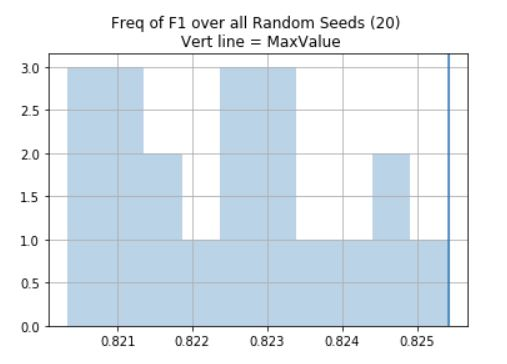
\includegraphics[width=0.75\textwidth]{seed_hist_f1}
	\caption{Histogram of F1 metric averaged across 5-fold metric}
	\label{fig:random_seed_hist}
\end{figure}

\subsection{Results}
Below in Table \ref{tab:tab_results} we layout three results from our submissions in the competition. The first is the baseline Naive Bayes SVM solution, with an F1 of 0.7548.  Second is our first random seed selected for the classifier which produces a 0.8083 result.  While better than the NB-SVM solution, we pick the best validation F1 from the 20 seeds we tried. This produced our final submission of 0.8099.
Note that applying this model over our validation set achieved an F1 of 0.8254 and a test set F1 of 0.8099 - a drop of 0.0155 in F1 for the true out-of-sample data.

\begin{table}[ht]
	% table caption is above the table
	\caption{Comparative Results}
	\label{tab:tab_results}
	\begin{tabular}{lllll}
		\hline\noalign{\smallskip}
		 & Accuracy & Precision & Recall & F1 \\
		\noalign{\smallskip}\hline\noalign{\smallskip}
NBSVM &      0.8223 & 0.8180 & 0.7007 & 0.7548 \\
First Seed & 0.8461 & 0.7869 & 0.8309 & 0.8083 \\
Best Seed &  0.8458 & 0.7806 & 0.8416 & \textbf{0.8099} \\
		\noalign{\smallskip}\hline
	\end{tabular}
\end{table}

\section{Conclusion}
\label{sec:5}
This paper describes our implementation of a neural net model for classification and regression in the HAHA 2019 challenge.  Our solution placed $3^{rd}$ in Task 1 and $2^{nd}$ in Task 2 in the final competition standings.  We describe the data collection, pre-training, and final model building steps for this contest.  Twitter has slang and abbreviations that are unique to the short-format as well as generous use of emoticons.  To capture these features, we collected our own dataset based on Spanish Tweets that is 16 times larger than the competition data set and allowed us to pre-train a langauge model.  Humor is subtle and using a label smoothed loss allowed us to not become too overconfident in our predictions and train more quickly without the gradual unfreezing required by ULMFiT. We have open-sourced all  code used in this contest to further enable research on this task in the future.

\section{other}


%%  Comment from Kyle:
%%Maybe you have some good advice to give other people related to points one and two of your main contributions, what do you think the primary benefit of transfer learning was - especially the use of tweets for the vocab and so on, versus the "standard" wikipedia? 
%
%Pretraining allows the model to get "close" to the right language model
%Pre-training uses a wider universe of language than just the model training set.  We have a better chance to predict the test-set data by leveraging additional data.
%
%%As for the label smoothing, what is your general insight on what settings of label smoothing worked well, why penalizing confident stuff was extra useful here?	
%%	For example in 4.2.1, why does label smoothing bypass gradual unfreezing? 
%
%With so many trainable params models can become focused on refining the prediiction on already correct predictions (going from .85 to .95 in the softmax output).  Gradual unfreezing prevents this kind of over-fitting by regularizing through restricting the params that can be fit.  Label smoothing achieves the same thing by preventing the maximum classification from becoming too large.  
%
%Manually built labels always lead to some errors.  there could be some that are only marginally funny, yet classified as "Humorous."  We don't want to be overconfident in our classification of these jokes, 
%and label smoothing helps us to overcome that noise. 
%
%
%Twitter has slang and abbreviations that are unique to the short-format as well as generous use of emoticons. 

\begin{acknowledgements}
The author would like to thank Kyle Kastner for his edits, suggestions and recommendations in writing up these results. 
\end{acknowledgements}


% Authors must disclose all relationships or interests that 
% could have direct or potential influence or impart bias on 
% the work: 
%
% \section*{Conflict of interest}
%
% The authors declare that they have no conflict of interest.


% BibTeX users please use one of
%\bibliographystyle{fullname}      % basic style, author-year citations

%\bibliographystyle{spbasic}      % basic style, author-year citations
\bibliographystyle{spmpsci}      % mathematics and physical sciences
%\bibliographystyle{spphys}       % APS-like style for physics
\bibliography{local}   % name your BibTeX data base

\end{document}
% end of file template.tex

